%
%	overview.tex
%
%	Project Details: Overview
%
%	John Hughes and Michael Jean
%	University of Manitoba
%

\section{Overview and Goals}

The vehicle as a whole is primarily a mechanical device, but carries several critical electronic 
control systems. Three key mechanical systems that either require electronic control or can benefit 
from electronic control are

\begin{itemize}
\item the \emph{internal combustion engine} (ICE\nomenclature{ICE}{Internal Combustion Engine}); 
\item the \emph{braking system}; and
\item the \emph{suspension system}.
\end{itemize}

\subsection{Internal Combustion Engine}

\nomenclature{MAP}{Manifold Absolute Pressure}
\nomenclature{ECU}{Engine Control Unit}
\nomenclature{DAQ}{Data Aquisition device, provides and logs high-performance GPS, accelerometer, and ADC input data}
\nomenclature{GPS}{Global Positioning System}

The ICE is the stock \emph{Honda CBR600F4i} motorcycle engine. It is a 600 cm$^3$ super-sport class engine with an internal 6-speed chain driven transmission. 

\begin{figure}[H]
	\centering
	 	\includegraphics[scale=0.5]{figures/cbr600f4i.png}
    \caption{The Honda CBR600F4i motorcycle.}
    \label{fig:cbr600f4i_cycle}
\end{figure}

The engine has a set of sensors attached to it, including

\begin{itemize}
\item an O$_{2}$ sensor;
\item a Manifold Absolute Pressure (MAP) sensor; 
\item an oil pressure sensor;
\item a water temperature sensor;
\item a throttle position sensor;
\item a gear position sensor;
\item cam and crank position sensors; and
\item an output shaft speed sensor.
\end{itemize}

Several tasks and responsibilites are best accomplished by electronic means, i.e.,

\begin{itemize}
\item the fuel injectors must be provided with timing signals;
\item the spark coils must be provided with firing signals;
\item a signal to engage the starter solenoid must be provided;
\item the clutch and gear selection levers must be intelligently actuated to change gears; 
\item the clutch must be intelligently actuated to enable the vehicle to move forward slowly;
\item the intake plenum valve must be opened or closed as driving conditions warrant; and
\item sensor outputs must be logged and relayed to team members wirelessly.
\end{itemize}

A specialized third-party component called the \emph{Engine Control Unit} (ECU) controls the 
fuel injector and spark coil systems that in turn control the combustion cycle of the engine. 
The particular model of ECU used by the Formula SAE car is the S80Pro from DTAFast \cite{s60pro}. 
The ECU uses the O$_{2}$, MAP, cam position, and crank position sensors to adjust the fuel injector 
and spark coil timings. This keeps the engine running smoothly. The ECU features a traction control 
system that monitors wheel slip and cuts spark and fuel to provide traction when one of the wheels 
is slipping. The ECU also collects the various sensor readings and makes them available to other
electronic devices at a fixed frequency through a shared data bus. 

\begin{figure}[H]
	\centering
	 	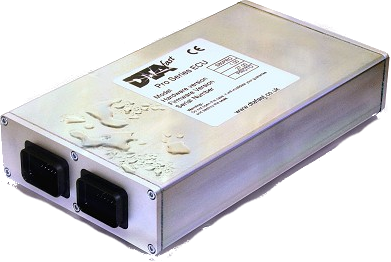
\includegraphics[scale=0.5]{figures/s80.png}
    \caption{The DTAFast S80Pro engine control unit.}
    \label{fig:s80pro_product}
\end{figure}

The ICE is started by energizing a \emph{starter solenoid}. This solenoid relays a large electric 
current to the \emph{starter motor}, which turns over the engine and causes it to start. An 
external control signal from the driver must engage and disengage the starter solenoid.

The ICE has an internal 6-speed manual transmission. The first, fifth, and sixth gears have been 
removed to reduce weight. The vehicle is not operated at speeds that would benefit from the presence 
of the fifth or sixth gear.

The clutch is actuated by a lever attached to the engine body. a pre-tensioned spring keeps the 
clutch engaged when there is no force on the lever. As force is applied to the lever, the clutch 
is gradually disengaged. The relationship between lever position the distance between the clutch 
plate and flywheel is non-linear. 

The gear selector is also acutated by a lever attached to the engine body. The gear selector may 
be rotated in either direction from its rest point. Up-shifting is accomplished by rotating the 
lever in one direction, while down-shifting is accomplished by rotating the lever in the opposite 
direction. 

Opearting a purely mechanical manual transmission is taxing on the driver, and requires
levers and linkages in the cockpit. Ideally, shifting between gears should happen as quickly 
as possible and require as little of the driver's attention as possible. Engagment of the clutch
should be as smooth as possible. 

The intake plenum valve controls the effective length of the intake runners. Longer intake runners
provide more air for combustion in the engine, which affects the air to fuel ratio and the
overall efficiency and performance of the engine.

Another specialized third-party component called the \emph{Data Aquisition Device} (DAQ) is used
to log and relay sensor data to other electronic devices.

The particular DAQ used is the model DL1 from Race Technology \cite{DL1Dsheet}. The DL1 is an 
expandable data logger with built-in 20-Hz GPS and 3-axis accelerometer. Race Technology provides 
a software suite that communicates with the DAQ using a documented serial protocol. Every item that 
the DAQ logs is output to its own channel in real time on the serial bus. It is also possible to 
configure the software to recognize new channels for arbitrary types of data. 

\begin{figure}[H]
	\centering
	 	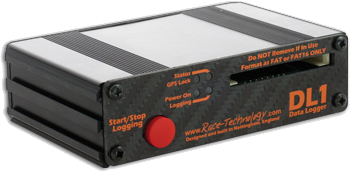
\includegraphics[scale=0.5]{figures/dl1.png}
    \caption{The Race Systems DL1 data acquisition device.}
    \label{fig:dl1_product}
\end{figure}

\subsection{Braking System}

The braking system on the 2010 Formula vehicle is a hydraulically-controlled, \emph{disc brake} 
system. Hydraulic pressure causes calipers on each wheel to squeeze friction pads against the 
discs, thus braking the vehicle. There are two entirely independant closed hydraulic systems, one 
for the front brakes and the other for the rear brakes. If one of the systems fails, the other 
system may be used to safely stop the vehice.

A brake pedal in the cockpit is used to engage the brakes. Two \emph{brake master cylinders}
(one for the front system and the other for the rear system) are connected to the brake pedal by 
way of a \emph{balance bar} (see figure \ref{fig:balance_bar_diag}). The balance bar distributes 
force from the brake pedal to the master cylinders \cite{TiltonBrakeBias}. 

Changing the relative braking force between the front and rear is called \emph{brake biasing}. 
For example, having 65\% of the braking force applied to the front wheels and 35\% to the rear is 
denoted as "65/35" brake biasing. 

Most of the vehicle weight is in the rear, where the engine is mounted. During braking, weight is 
effectively transferred from the rear of the vehicle to the front. This weight transfer reduces the 
braking force available to the rear tires. If too much rear brake force is applied, the rear tires 
may lock-up and the vehicle will lose traction \cite{FundVehicleDynamics}. This situation can be avoided
by properly biasing the brakes for driving conditions.

\begin{figure}[h!]
	\centering
	 	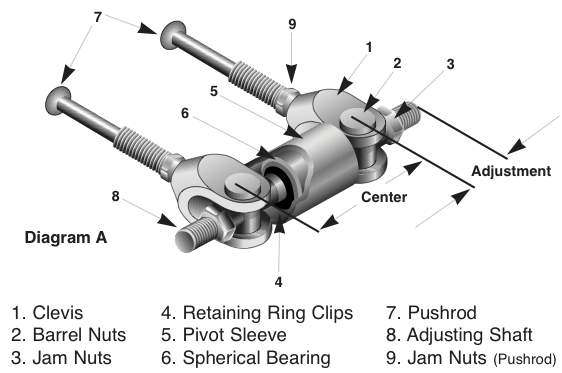
\includegraphics[scale=1.0]{figures/balance_bar_diag.png}
    \caption{A Tilton brand balance bar, similar to that used on the Formula SAE vehicle.}
    \label{fig:balance_bar_diag}
\end{figure}

The relative force provided to each brake master cylinder can be changed by rotating an 
\emph{adjusting shaft} on the balance bar. When the adjusting shaft is centered between 
the front and rear cylinders, an equal amount of force will be applied to each. The relationship 
between the deviation of the adjusting shaft from it's centre position and the relative force 
applied to each cylinder is approximately linear for a range between 65/35 and 35/65. See table 
\ref{table:bb_force_distribution} for more details.

\begin{table}[H]
	\centering
	\caption{Braking force distribution}
	\label{table:bb_force_distribution}	
	\begin{tabular}{| l | c | c |}
		\hline Adjustment Rod Position & Left Clevis & Right Clevis  \\ \hline
		\hline 3/8" left-of-centre & 65\% & 35\% \\ 
		\hline 1/4" left-of-centre & 60\% & 40\% \\
		\hline 1/8" left-of-centre & 55\% & 45\% \\
		\hline Centred & 50\% & 50\% \\
		\hline 1/8" right-of-centre & 45\% & 55\% \\
		\hline 1/4" right-of-centre & 40\% & 60\% \\
		\hline 3/8" right-of-centre & 35\% & 65\% \\
		\hline
	\end{tabular}
\end{table}

Manually adjusting the brake bias is an arduous task. The brake pedal and master cylinders are 
attached to a \emph{brake pedal assembly} located at the end of the cockpit (see figures
\ref{fig:brake_pedal_assy_a} and \ref{fig:brake_pedal_assy_b}). This assembly is very difficult to 
reach by hand, and there is very little room to work. Removal of the brake pedal assembly is 
prohibited because the brake lines that connect to the master cylinder cannot be removed without 
depressurizing both the front and rear brake systems. The adjustment rod is rotated with an allen 
key. Precise adjustment requires calipers, and is nearly impossible given the cramped space available.

\begin{figure}[h!]
	\centering
		\subfloat[Front view]{
			\label{fig:brake_pedal_assy_a}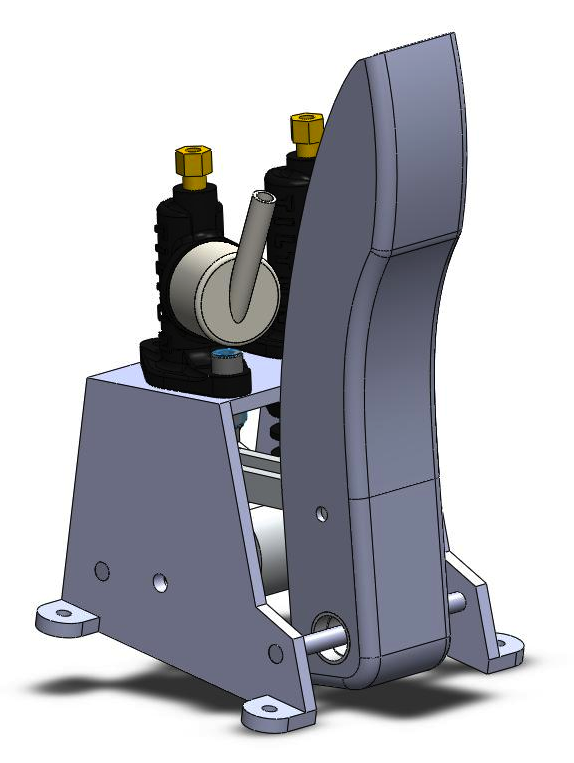
\includegraphics[scale=0.4]{figures/brake_pedal_assy_a.png}}
		\subfloat[Rear view]{
			\label{fig:brake_pedal_assy_b}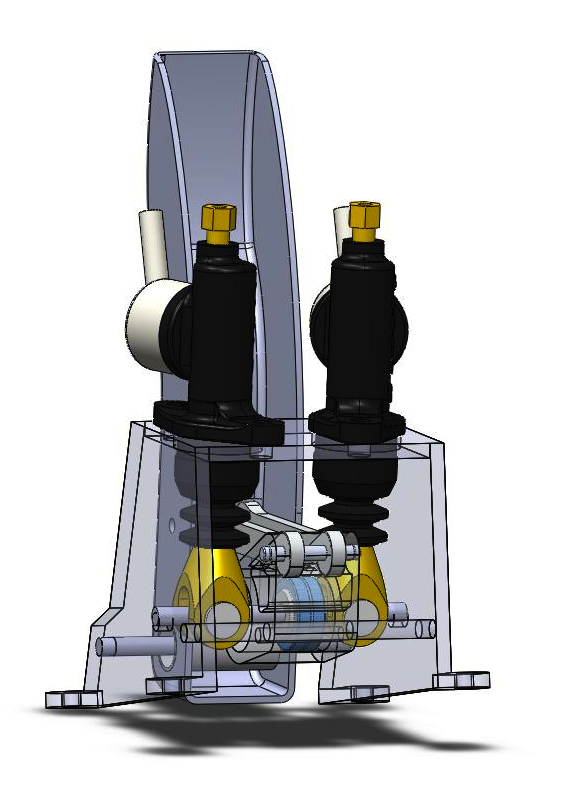
\includegraphics[scale=0.4]{figures/brake_pedal_assy_b.png}}
    \caption{The brake pedal assembly.}
    \label{fig:brake_pedal_assy}
\end{figure}

\subsection{Suspension System}

The suspension system consists of springs that control the height and attack of the vehicle. 
Although electronic control of the suspension system is desirable, it is out of the scope of
our thesis project and will be approached by future UMSAE teams.



